\section{Introduction}
Modern software systems involve intricate changes that extend far beyond source code modifications. A significant portion of system behavior is governed by configuration files, encompassing deployment scripts, service settings, infrastructure definitions, and more. Ensuring the correctness of these configurations is critical, yet challenging. Although software vendors often provide extensive manuals to guide administrators, the length and complexity of these documents can be prohibitive, frequently leading practitioners to resort to guesswork when configuring systems \cite{Xiang.2020}. This challenge is compounded by the rapid pace of technological evolution, which necessitates constant updates to configuration schemes.

The consequences of misconfiguration can be severe, significantly contributing to production bugs and system failures, as highlighted by large-scale studies \cite{Tang.2015}. Traditionally, validating configurations has relied on methods such as static analysis, integration testing, and manual review \cite{Lian.2024}. While valuable, these approaches often struggle to keep pace with the complexity and dynamism of modern software environments. Furthermore, the scale at which validation is required can be immense; Facebook, for example, reported executing trillions of configuration checks daily \cite{Tang.2015}. This necessitates solutions that are not only accurate but also highly performant and resource-efficient, implying that evaluation solely based on metrics like precision or recall is insufficient. Consequently, there is a pressing need for more automated, reliable, and scalable validation techniques.

Retrieval-Augmented Generation (RAG) systems offer a promising approach to address this gap. By combining the knowledge retrieval capabilities of search systems with the reasoning power of Large Language Models (LLMs), RAG can potentially interpret complex technical documentation (like configuration manuals) and apply this understanding to validate specific configurations against best practices or requirements.

This chapter aims to demonstrate the practical application of the RAGBench evaluation framework, detailed in Chapter 4, to the specific problem of configuration validation. We will leverage this framework to systematically evaluate the performance of various RAG configurations against established baselines using an extended version of the CTest dataset \cite{Lian.2024}, which includes synthetically generated examples. While acknowledging that configuration validation is a multifaceted problem involving aspects like inter-configuration dependencies, this experiment focuses specifically on validating individual configuration settings based on documented guidelines.

The remainder of this chapter is structured as follows: Section \ref{sec:related_works_exp} discusses related work in applying RAG to software engineering tasks, particularly configuration validation. Section \ref{sec:exp_design_exec} details the experiment design, including the dataset, baselines, RAG configurations, evaluation metrics, and tools used, adhering to the methodology outlined in Chapter 4. Section \ref{sec:exp_results} presents and analyzes the results obtained on the validation and test sets, including end-to-end performance, component analysis, and failure analysis. Section \ref{sec:exp_discussion} discusses the overall findings and their implications. Finally, Section \ref{sec:exp_conclusion} summarizes the key outcomes of the experiment.
% Note: Added \label tags for section references - adjust as needed if you rename sections.

\section{Related Works} \label{sec:related_works_exp}
Several approaches have been developed for validating software configurations.

Specification-based frameworks, such as ConfValley \cite{Huang.2015}, function by having engineers define validation rules explicitly, often in a declarative manner. Configuration Testing validates configuration values by executing the software components that use these values and observing the resulting program behavior \cite{XudongSun.2020}. This method is used to detect the dynamic effects of configuration settings and identify errors.

Lian et al. \cite{Lian.2024} introduced Ciri, a method that uses Large Language Models for configuration validation. Ciri employs prompt engineering and few-shot learning, providing the LLM with examples of both valid and invalid configurations alongside relevant documentation snippets to identify misconfigurations. This work applies Retrieval-Augmented Generation to the configuration validation task presented by Lian et al. \cite{Lian.2024}. We utilize the RAGBench evaluation framework, detailed in Chapter \ref{chap:design}, to systematically assess and reconfigure different RAG systems. The aim is to optimize their performance for this specific task through iterative refinement.

\section{Experiment Design and Execution} \label{sec:exp_design_exec}
The following sections detail the design and execution of our configuration validation experiment. This experiment adheres strictly to the methodology established by the RAGBench framework presented in Chapter \ref{chap:design}. The core principle is to split the evaluation dataset into validation and test sets. All system configuration, evaluation, and iterative refinement are performed exclusively on the validation set. Finally, generalization is assessed on the held-out test set. Specifically, we employed a 70/30 validation-test split for the extended CTest dataset to ensure a sufficiently large test set for estimating generalization error (as discussed in Section \ref{sec:valtestsplit}).

Our experimental workflow begins by establishing performance baselines using a standalone LLM and a naive RAG system (Section \ref{sec:e2e}). We then evaluate an initial RAG configuration. Subsequent steps involve analyzing performance bottlenecks and failures using the framework's end-to-end and component-level metrics, alongside detailed trace analysis facilitated by MLflow and Langfuse (Section \ref{sec:ui}). Insights from this analysis guide iterative reconfiguration cycles aimed at improving performance on the validation set.

A key difference in our evaluation approach compared to the original Ciri experiment \cite{Lian.2024} lies in handling output formatting. While Ciri reran queries until a correctly formatted answer was obtained, our framework employs a strict format check; if the generator's output does not conform to the expected format (such as providing a clear "valid" or "invalid" classification with reasoning), the response is marked as incorrect. This reflects a scenario where automated post-processing requires predictable output.


\subsection{Experimental Setup} \label{sec:exp_setup}
The experiments were conducted using the computational resources specified below. A dedicated server hosted by Hetzner served as the primary environment for running the evaluation framework, encompassing data processing, baseline evaluations, and RAG pipeline executions that involved API-based LLMs or CPU-based components. We selected both closed and open-source models and utilized \\OpenRouter.ai \cite{openrouter-inc-2023} for all API requests. We opted not to self-host models, as this could skew system metrics such as latency.

We chose the CCX23 dedicated CPU server\cite{hetzner-online-gmbh-2025} for all our tests
\begin{itemize}
    \item VCPU: 4
    \item RAM: 16 GB
    \item SSD: 160 GB
\end{itemize}

We also used runpod.io\cite{runpod-2025} and deployed a RTX 4090 with 24GB VRAM for our experiments with vllm \cite{Kwon.12.09.2023} embedding models.

\paragraph{Dataset} 
We used the CTest dataset, prepared by the team behind Ciri \cite{Lian.2024}\cite{xlab-uiuc-2025}. The data consists of real-world misconfiguration scenarios, augmented with synthetic data. We had 907 test cases in total. The distribution per system is shown in the following table.

\begin{table}[h]
    \centering
    \begin{tabular}{|l|c|c|}
        \hline
        \textbf{Technology} & \textbf{Number of Files} & \textbf{Version} \\
        \hline
        alluxio & 111 & 2.5.0 \\
        django & 36 & 4.0.0 \\
        etcd & 64 & 3.5.0 \\
        hbase & 107 & 2.2.7 \\
        hcommon & 138 & 3.3.0 \\
        hdfs & 149 & 3.3.0 \\
        postgresql & 62 & 13.0 \\
        redis & 88 & 7.0.0 \\
        yarn & 80 & 3.3.0 \\
        zookeeper & 72 & 3.7.0 \\
        \hline
    \end{tabular}
    \caption{Evaluation Dataset: Number of configuration files and versions per system.}
    \label{tab:technology_values}
\end{table}

We then defined the validation-test split parameter. We chose a test size of 20 \%, resulting in 725 validation data points and 182 test data points.  

The ingestion of data into our vector database required scraping official documentation for each specific version. However, we could not find documentation or a manual for this specific Redis version as well as for HBase, HCommon, and HDFS. Table \ref{tab:technology_documentation} shows the documentation sources we scraped.

\begin{table}[h]
    \centering
    \begin{tabular}{|l|l|}
        \hline
        \textbf{Technology (Version)} & \textbf{Documentation Page} \\
        \hline
        alluxio (2.5.0) & \texttt{https://docs.alluxio.io/os/javadoc/2.5/} \\
        django (4.0.0) & \texttt{https://docs.djangoproject.com/en/4.0/} \\
        etcd (3.5.0) & \texttt{https://etcd.io/docs/v3.5/} \\
        \textbf{hadoop-} & \texttt{https://hadoop.apache.org/docs/stable/}\\
        & \hspace{0.25cm} \texttt{hadoop-project-dist/} \\
        \hspace{0.15cm} hbase (2.2.7) & \hspace{0.5cm} \texttt{hadoop-common/} \\
        \hspace{0.15cm} hcommon (3.3.0) & \hspace{0.5cm} \texttt{hadoop-common/} \\
        \hspace{0.15cm} hdfs (3.3.0) & \hspace{0.5cm} \texttt{hadoop-hdfs/} \\
        postgresql (13.0) & \texttt{https://www.postgresql.org/docs/13/} \\
        redis (7.0.0) & \texttt{https://redis.io/docs/latest/commands/} \\
        yarn (3.3.0) & \texttt{https://hadoop.apache.org/docs/r3.3.0/} \\
        zookeeper (3.7.0) & \texttt{https://zookeeper.apache.org/doc/r3.7.0} \\
        & \hspace{0.25cm} \texttt{/apidocs/zookeeper-server/} \\
        \hline
    \end{tabular}
    \caption{Technology and Documentation Links: Starting at those documentation pages as base URLs, we scraped every linked page with the same base URL as a prefix recursively.}
    \label{tab:technology_documentation}
\end{table}

Data ingestion was performed ad hoc before each experiment to ensure comparable results for ingestion times.

\subsection{Reconfiguration Phases} \label{sec:exp_results} 

\paragraph{Initial Configuration and Baselines} \label{sec:exp_initial_config}
We used several baselines for comparison. Initially, we ran our experiment with the baselines defined in Section \ref{chap:design}: a standalone LLM and a predefined minimal RAG system with BM25 sparse retrieval. For both baselines, we used OpenAI's GPT-4o-mini \cite{OpenAI_2022}. The standalone system consists of only a generator and an answer builder for extracting "valid" or "invalid" from the generated output. The second baseline adds a retriever immediately before the generator and lists the top-10 documents without any pre- or postprocessing. These basic architectures allow us to determine if complex adjustments improve validator quality.

We also rebuilt the Ciri system within our Haystack RAG architecture and used it as a baseline. As we only used our framework for running evaluations, there are some minor differences in methodology due to implementation limitations. We did not look at the results per system, which means that we do not have knowledge of whether our system works better for Django or Alluxio systems. However we could run for each system a separate experiment, but we chose against it for better comparability of the final result and cost reduction of the experiment. We also did only evaluate file-level validation. Ciri used few-shot examples with a number of valid and invalid configurations. We did not vary the number of valid or invalid shots; instead, we have chosen the best performing configuration with one valid and three invalid shots. Lastly, Ciri used several language models for its experiments. We were limited to using \textit{gpt-3.5-turbo-0125}\cite{OpenAI_2022}. Other models were either unavailable, because the used version is outdated, continuously trained or too expensive for the experiment to run with our budget. However, we achieved a F1-Score of \textit{0.680} which close to the Ciri reported F1-Score of \textit{0.720}. The pipeline figures can be found in the appendix.

\subparagraph{Initial RAG Configuration} 
First, we tested different standalone LLMs for measuring the performance of LLMs without complex system architecture. For our evaluation, we chose Qwen's \textit{QwQ-32B} \cite{qwq32b} and \textit{Qwen-2.5-coder-32b-instruct} \cite{hui2024qwen2}\cite{qwen2}\cite{qwen2.5}, OpenAI's versioned \textit{o1-mini}, an earlier version of \textit{gpt-4o-mini} (\textit{gpt-4o-mini-2024-08-06}), and an up-to-date version of \textit{gpt-4o-mini} for comparison. We also tested OpenAI's web-search version of \textit{gpt-4o-mini}, which appears to be an out-of-the-box RAG-system \cite{OpenAI_2022}. Lastly we added DeepSeek's most recent model \textit{V3} \cite{deepseekai2024deepseekv3technicalreport} to the list. 

\begin{figure}[!ht]
    \centering
    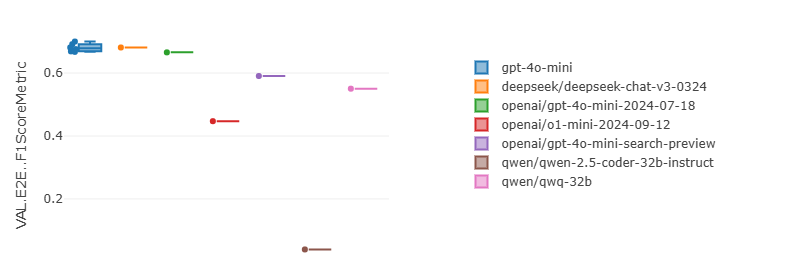
\includegraphics[width=0.95\textwidth]{images/LLMStandalone-by-model.png}\\[6pt]
    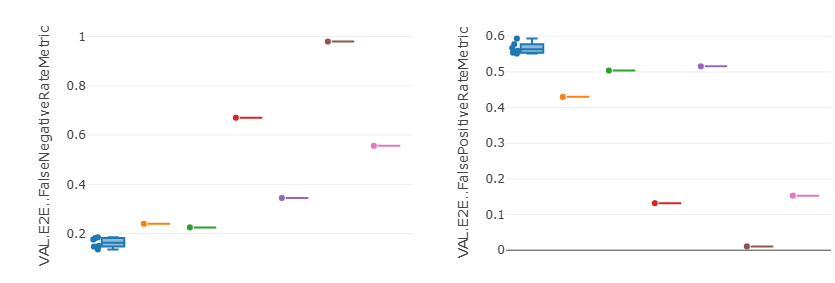
\includegraphics[width=\textwidth]{images/LLMStandalone-by-model-FNRFPR.png}
    \caption{(Upper) F1-Scores for standalone Large Language Models on the configuration validation task. (Lower) False-Negative Rate (Left) and False-Positive Rate (Right) for the standalone LLMs on the configuration validation task.}
    \label{fig:LLMStandalone-Results}
  \end{figure}

Results can be seen in Figure \ref{fig:LLMStandalone-Results}. The most recent \textit{GPT-4o-mini} model performs best for F1-Score. The evaluated models differ more strongly on False-Positives Rate and False-Negative Rate than on F1-Scores. \textit{GPT-4o-mini} has the lowest False-Negative-Rate and the highest False-Positive-Rate. Since positives represent valid configurations, \textit{GPT-4o-mini} classifies invalid configurations as valid more often, and conversely, classifies valid configurations as invalid less frequently. The older version of \textit{GPT-4o-mini} from 2024 and the web-search model have a slightly worse F1-Score, but more balanced FNR and FPR metrics. Even without few-shot learning as done by the Ciri team, the most recent version of \textit{gpt-4o-mini} did score a slightly higher average F1-Score ($0.681$) than the configuration from the Ciri team with \textit{gpt-3.5-turbo-0125} ($0.680$). In contrast to other models, we ran the most recent version of gpt-4o-mini more frequently as baseline in later experiment runs. The variance in F1-Scores in those runs is relatively small ($1.41 \cdot 10^{-5}$).


  Next, beyond the basic BM25 retriever (predefined as a baseline), we evaluated additional retrieval configurations. First, we tested a configuration employing only a dense retriever with OpenAI's \textit{text-embedding-3-small} \cite{OpenAI_2022}. Second, we implemented a hybrid retrieval configuration. This hybrid approach combined the results from the BM25 retriever and the aforementioned dense retriever, using three different weighting schemes for their respective scores: (1:2), (1:1), and (2:1), where the ratios represent (BM25 score : Dense score). We have evaluated the performance of these configurations with both the \textit{gpt-4o-mini-2024-08-06} and the most recent \textit{gpt-4o-mini} model. The results can be seen in Figure \ref{fig:conf-phase-0-retrievers}. The results show that the selected model has more impact on the overall performance than the retrieval technique in this experiment. The retrieval metrics can be seen in Table \ref{tab:retrieval_metrics}. Overall, the sparse retriever performed better than the dense retriever. Both retrieval techniques performed poorly on retrieval quality. The weight distribution of the hybrid retriever had only a small impact on the performance, with F1-Score ranging from \textit{0.567} to \textit{0.582}.

\begin{table}[!ht]
    \centering
    \begin{tabular}{|l|c|c|}
        \hline
        \textbf{Metric} & \textbf{BM25} & \textbf{Dense} \\
        \hline
        ContextRelevance & 0.396 & 0.176 \\
        MAP@K & 0.096 & 0.030 \\
        \hline
    \end{tabular}
    \caption{Retrieval metrics comparison between BM25 and Dense retrieval}
    \label{tab:retrieval_metrics}
\end{table}

\begin{figure}[!ht]
    \centering
    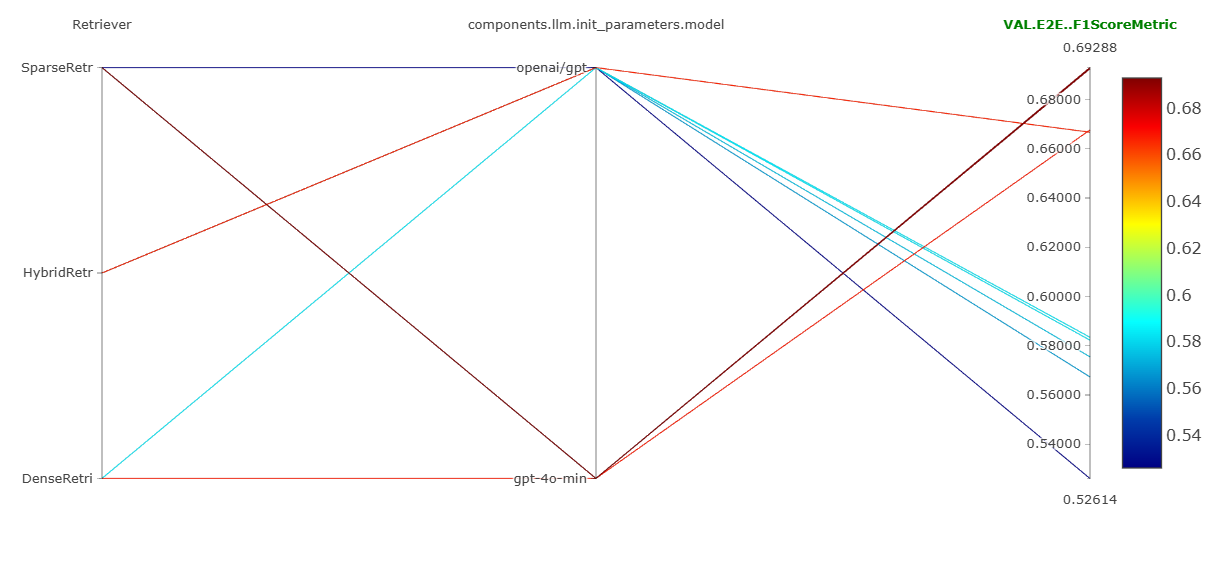
\includegraphics[width=\textwidth]{images/RetrievalTypes-vs-LLM-f1.png}\\[6pt]
    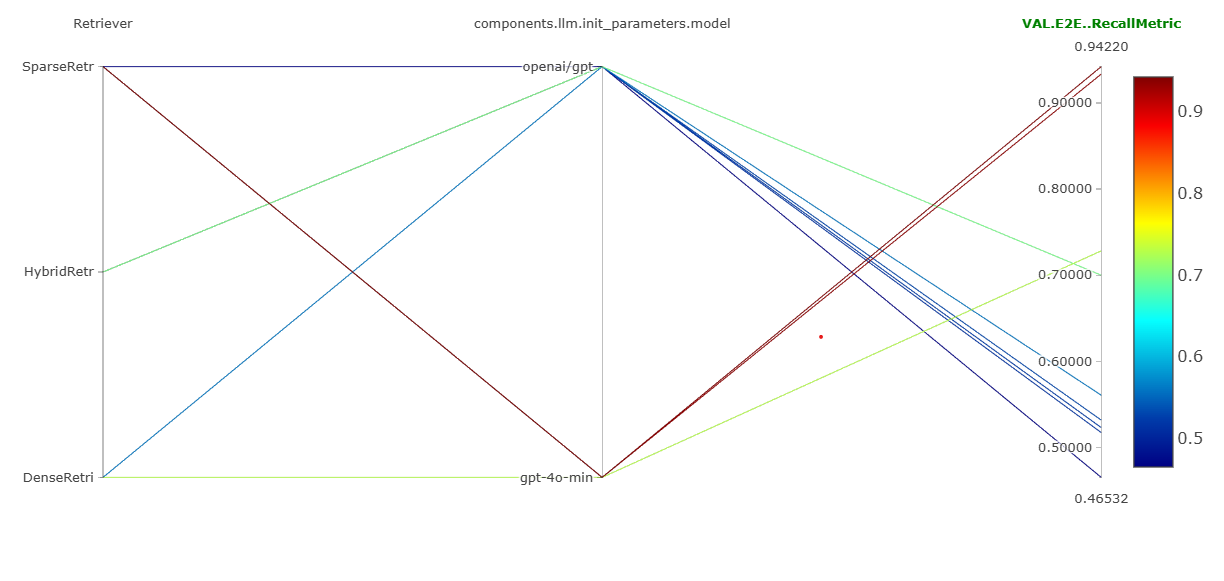
\includegraphics[width=\textwidth]{images/RetrievalTypes-vs-LLM-Recall.png}
    \caption{Experiments with different retrieval techniques and models. In both figures the upper model is the \textit{gpt-4o-mini-2024-08-06} model and the lower model is the most recent \textit{gpt-4o-mini}. The upper figure shows the F1-score and the lower one shows the recall score.}
    \label{fig:conf-phase-0-retrievers}
\end{figure}

Following this phase, we attempted to improve the resource quality of the data. The scraped documentation HTML files were extensively cleaned by removing numerous elements irrelevant to configuration parameters. This included structural page elements (headers, footers, navigation bars, sidebars), presentational tags (styles, SVGs, images), and embedded code (scripts). We removed all of these elements and only kept the relevant ones containing text or metadata. The cleanup statistics can be seen in Table \ref{tab:cleanup_stats}. However, the retrieval quality for sparse retrievers did unexpectedly decrease from \textit{0.693} to \textit{0.567}. 

\begin{table}[h]
    \centering
    \begin{tabular}{|l|r|r|r|r|}
        \hline
        \textbf{System} & \textbf{Files} & \textbf{Original Size} & \textbf{New Size} & \textbf{Reduction} \\
        \hline
        alluxio & 230 & 20.64MB & 19.58MB & 5.16\% \\
        django & 634 & 37.10MB & 22.05MB & 40.57\% \\
        etcd & 113 & 19.27MB & 1.86MB & 90.33\% \\
        hbase & 440 & 26.42MB & 18.30MB & 30.74\% \\
        hdfs & 108 & 2.83MB & 2.09MB & 26.18\% \\
        postgresql & 1137 & 26.50MB & 22.94MB & 13.43\% \\
        redis & 515 & 93.69MB & 8.33MB & 91.11\% \\
        yarn & 563 & 40.93MB & 27.43MB & 32.99\% \\
        zookeeper & 35 & 2.29MB & 2.12MB & 7.45\% \\
        \hline
        \textbf{TOTAL} & \textbf{3775} & \textbf{269.68MB} & \textbf{124.70MB} & \textbf{37.55\%} \\
        \hline
    \end{tabular}
    \caption{HTML Documentation Cleanup Statistics}
    \label{tab:cleanup_stats}
\end{table}

As the results were not improving, we felt forced to change more parameters within a configuration step. Therefore, for the dense retriever, in addition to using the improved quality data, we also tried a different embedding model. We used the \textit{infly/inf-retriever-v1-1.5b} \cite{inflyai2025} model, because it is small enough for self-hosting and scores best in its size class in the MTEB \cite{muennighoff2022mteb} \cite{MTEB} in category "Code". We also applied a 4R-architecture with rewriter that rewrites the configuration question to be validated into hypothetical documentation pages so that the embedded retriever could in theory map those hypothetical documents with the real ones in the embedded space. Lastly, we added a Lost-in-the-middle reranker \cite{Liu.06.07.2023}. The results improved greatly, achieving an F1-Score of \textit{0.6825}, which exceeded the results we measured for Ciri. 


Lastly, we wanted to update Ciri's results with more recent state-of-the-art models. Therefore, we tested the Ciri configuration with the models \textit{gpt-4o-mini-2024-08-06} and the most recent version of \textit{gpt-4o-mini} \cite{OpenAI_2022}. We also used \textit{gemini-2.5-flash} \cite{gemini-2.0}, \textit{deepseek-chat-v3-0324} \cite{deepseekai2024deepseekv3technicalreport}, and the models from Alibaba released in April 2025: \textit{qwen3-32b} and \textit{qwen3-235b-a22b} \cite{qwen3}. We evaluated these models in two different scenarios: one without explicit reasoning before answering the question and one with reasoning before answering the question. 

% Add this to your preamble:
% \usepackage{multirow}

\begin{table}[h]
    \centering
    \begin{tabular}{|l|c|c|c|c|c|c|}
        \hline
        \textbf{Model} & \multicolumn{3}{c|}{\textbf{Without Reasoning}} & \multicolumn{3}{c|}{\textbf{With Reasoning}} \\
        \hline
        & \textbf{F1} & \textbf{P} & \textbf{R} & \textbf{F1} &  \textbf{P} & \textbf{R} \\
        \hline
        gpt-4o-mini             & 0.688 & 0.785 & 0.613 & 0.508 & 0.796 & 0.373 \\
        gpt-4o-mini-2024-08-06  & 0.699 & 0.784 & 0.630 & 0.501 & 0.776 & 0.370\\
        gemini-2.5-flash        & 0.747 & 0.806 & 0.697 & 0.456 & 0.829 & 0.315 \\
        deepseek-chat-v3-0324   & \textbf{0.776} & 0.794 & \textbf{0.759} & 0.666 & 0.790 & 0.575 \\
        qwen3-32b & 0.609 & 0.810 & 0.488 & 0.603 & \textbf{0.841} & 0.470 \\
        qwen3-235b-a22b$^1$ & - & - & - & - & - & - \\
        \hline
    \end{tabular}
    \caption{Comparison of model performance (F1-Score, Precision (P), and Recall (R)) with and without explicit reasoning. $^1$Results for Qwen-3's Mixture-of-Experts model \textit{qwen3-235b-a22b} are incomplete due to errors on many queries; they are included for transparency}
    \label{tab:model_comparison}
\end{table}

Reasoning generally decreased the F1-score and recall across the tested models. The impact on precision scores was more varied: three models (\textit{gpt-4o-mini}, \textit{gemini-2.5-flash}, and \textit{qwen3-32b}) showed an increase in precision with reasoning, while two (\textit{gpt-4o-mini-2024-08-06} and \textit{deepseek-chat-v3-0324}) exhibited a slight decrease. This indicates that while prompting for reasoning consistently lowered recall (identifying fewer of all actual valid configurations), its effect on the precision of those classifications (the proportion of 'valid' classifications that were correct) was model-dependent.

The highest F1-Score (0.776) was achieved by the \textit{deepseek-chat-v3-0324} model within the Ciri configuration. Overall, we achieved good, though not matching, results (0.693) with a sparse configuration with the most recent version of \textit{gpt-4o-mini}. We also came close to this result with a dense 4R-architecture and the \textit{infly/inf-retriever-v1-1.5b} embedder (0.683). 



\subsection{Generalization Test} \label{sec:exp_generalization}
% Present the results of the final selected configuration(s) on the held-out test set (Sec 4.1, Sec 4.6).
% Compare test set performance against validation set performance for these configurations.
% Use tables/figures.
% Discuss any significant differences and potential signs of overfitting.

In this section, we address the generalization error for our experiments. Theoretically, generalization error occurs when parameters are tuned to best fit the evaluation data rather than the underlying problem. During our reconfiguration phases, we had limited success with RAG configurations. Typically, one would identify an effective combination of resources and configuration to address the problem, then fine-tune parameters to achieve the best-performing setup, which would subsequently be tested for generalization error. However, we did not achieve RAG configurations successful enough to warrant such a generalization test focused on overfitting from our tuning.

Instead, we decided to perform tests on the held-out test set using the best-performing models from Table \ref{tab:model_comparison} within the Ciri few-shot configuration. While this does not primarily test for generalization error stemming from our own parameter fine-tuning (as these specific model configurations were not iteratively tuned by us), it provides a valuable estimation of their performance variance on unseen data. This helps assess the consistency of these standalone LLM setups in this task. We selected \textit{deepseek-chat-v3-0324}, \textit{gemini-2.5-flash}, and the original Ciri configuration with \textit{gpt-3.5-turbo} for this purpose. 

\begin{table}[h]
    \centering
    \begin{tabular}{|l|c|c|c|c|c|c|}
        \hline
        \textbf{Model} & \multicolumn{3}{c|}{\textbf{Validation Set}} & \multicolumn{3}{c|}{\textbf{Test Set}} \\
        \hline
        & \textbf{F1} & \textbf{P} & \textbf{R} & \textbf{F1} &  \textbf{P} & \textbf{R} \\
        \hline
        gpt-3.5-turbo          & 0.680 & 0.735 & 0.633 & 0.650 & 0.663 & 0.639 \\
        gemini-2.5-flash       & 0.747 & 0.806 & 0.697 & 0.735 & 0.735 & 0.735 \\
        deepseek-chat-v3-0324  & \textbf{0.776} & 0.794 & \textbf{0.759} & 0.763 & 0.733 & 0.795 \\
        % qwen3-32b              & 0.609 & 0.810 & 0.488 & 0.647 & 0.827 & 0.531 \\
        \hline
    \end{tabular}
    \caption{Comparison of model performance between validation and test sets with F1-Score, precision (P) and recall (R).}
    \label{tab:generalization_comparison}
\end{table}



\subsection{System Metrics}

First, we present the different indexing times for the two embedding models that we tested. Figure \ref{fig:indexing-time} shows both the OpenAI embedding via API and the vLLM embedding via a runpod.io deployment. OpenAI's embedding API required 3.5 times more time for indexing.

\begin{figure}[!ht]
    \centering
    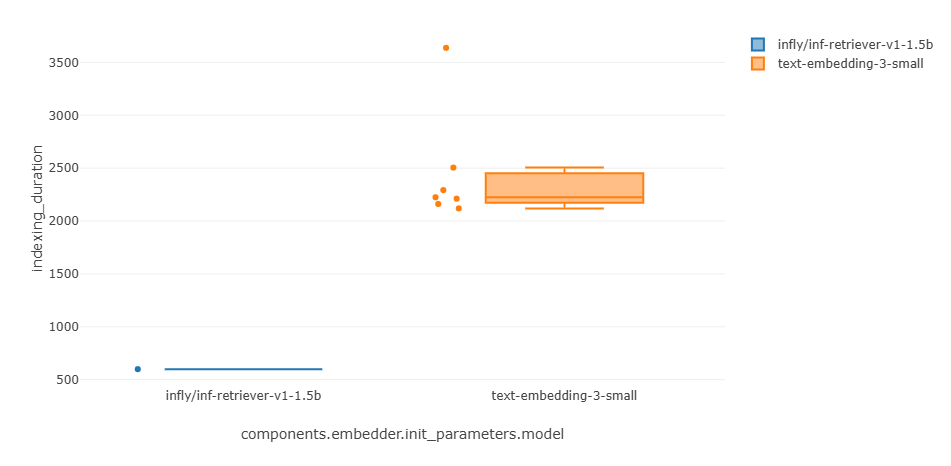
\includegraphics[width=\textwidth]{images/indexing-time.png}
    \caption{Indexing duration comparison between the two tested embedding models: \textit{openai/text-embedding-small-3} and \textit{infly/inf-retriever-v1-1.5b}.}
    \label{fig:indexing-time}
\end{figure}

We also measured the evaluation time to assess the usability implications of different RAG systems. The objective was to determine whether the performance boost offered by a RAG system justifies the potential drawback of longer computation times compared to simpler approaches. Since the best-performing configurations identified in our experiments were based on standalone LLMs using the Ciri few-shot approach (rather than more complex RAG pipelines), these top-performing systems were also inherently among the fastest in terms of computation time. As clearly shown in Figure \ref{fig:evaluation-time}, using a retriever of any type substantially increases computation times compared to the standalone LLM baseline (excluding data ingestion time). 

\begin{figure}[!ht]
    \centering
    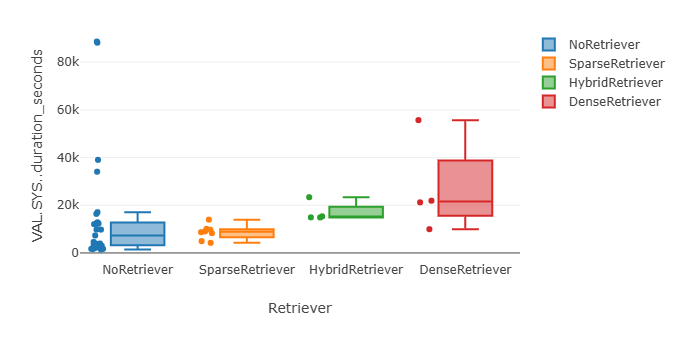
\includegraphics[width=\textwidth]{images/duration-retriever.png}
    \caption{Evaluation duration comparison between different retriever types (Sparse, Dense, Hybrid) and the standalone LLM baseline (No Retriever).}
    \label{fig:evaluation-time}
\end{figure}

We also measured system memory usage (e.g., peak RAM) to estimate the operational cost associated with deploying different configurations. Results are shown in Figure \ref{fig:memory}. Configurations involving hybrid and dense retrievers required the most RAM.

\begin{figure}[!ht]
    \centering
    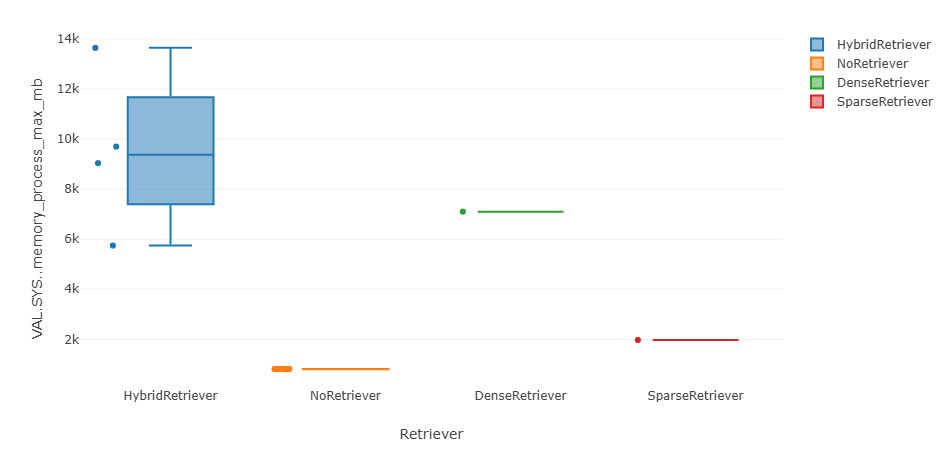
\includegraphics[width=\textwidth]{images/Max MB RAM.png}
    \caption{Comparison of maximum memory usage for different retriever types (Sparse, Dense, Hybrid) and the standalone LLM baseline (No Retriever).}
    \label{fig:memory}
\end{figure}

Lastly, we consider the costs associated with the models and embeddings. It was not possible to gather exact per-token costs paid through OpenRouter due to reporting incompatibilities with Haystack. However, all models processed a similar volume of input tokens, which was the primary driver of API costs. The output consisted only of the classification and a brief justification. Therefore, Table \ref{tab:model_costs} lists the advertised costs per million tokens for the evaluated models.

\begin{table}[!ht]
    \centering
    \caption{Cost comparison of different models per million tokens, grouped by provider}
    \label{tab:model_costs}
    \begin{tabular}{lrr}
        \hline
        \textbf{Model Name} & \textbf{Input (\$/M)} & \textbf{Output (\$/M)} \\
        \hline
        \multicolumn{3}{l}{\textit{OpenAI}} \\
        openai/gpt-3.5-turbo-0125 & 0.50 & 1.50 \\
        openai/gpt-4o-mini & 0.15 & 0.60 \\
        openai/gpt-4o-mini-2024-07-18 & 0.15 & 0.60 \\
        openai/gpt-4o-mini-search-preview & 0.15 & 0.60 \\
        openai/o1-mini-2024-09-12 & 1.10 & 4.40 \\
        \hline
        \multicolumn{3}{l}{\textit{Qwen}} \\
        qwen/qwen3-235b-a22b & 0.10 & 0.10 \\
        qwen/qwen3-32b & 0.10 & 0.30 \\
        qwen/qwen-2.5-coder-32b-instruct & 0.06 & 0.18 \\
        qwen/qwq-32b & 0.15 & 0.20 \\
        \hline
        \multicolumn{3}{l}{\textit{Google}} \\
        google/gemini-2.5-flash-preview & 0.15 & 0.60 \\
        \hline
        \multicolumn{3}{l}{\textit{DeepSeek}} \\
        deepseek/deepseek-chat-v3-0324 & 0.27 & 1.10 \\
        \hline
    \end{tabular}
\end{table}

Estimating the cost of embedding is more complex. First, consider the OpenAI API costs for \textit{text-embedding-small-3}. One run on the validation dataset (725 samples) processed approximately 9 million tokens (including ingestion and query embeddings). At a list price of \$0.02 per million tokens, this resulted in a cost of approximately \$0.18 for the run. For the self-hosted vLLM embedding, we consider the compute time. The initial indexing took approximately 598 seconds. At \$0.69 per hour for the runpod.io instance, this equates to approximately \$0.11 for ingestion. However, unlike token-based pricing where indexing dominates, for time-based instance pricing, the total experiment duration is the primary cost driver, as the instance must remain active to embed each query prior to retrieval. Since the relevant experiment run took 6.1 hours, the estimated total cost for using the vLLM embedding was \$4.21.




\section{Discussion} \label{sec:exp_discussion}
% Interpret the overall results of the experiment.
% Which configuration performed best overall?
% Did the RAG systems outperform the baselines?
% Was the added complexity of advanced RAG justified?
% Discuss the implications of the findings for the specific task (configuration validation).
% Acknowledge limitations of the experiment (e.g., dataset size, scope of configurations tested).

We used several standalone models with the initial prompt design. The model specifically designed for coding, \textit{Qwen-2.5-coder-32b-instruct}, performed poorly. We can see that the more recent models like the most recent version of gpt-4o-mini, Google's \textit{gemini-2.5-flash} or DeepSeek's \textit{deepseek-chat-v3-0324} had a higher F1-score than other older models like Qwen's QwQ-32B. Reasoning did not improve results in our scenario. This might be attributable to the fact that we did not use the models' native reasoning capabilities, but rather prompted for artificial reasoning before the final answer. Error analysis showed that reasoning lead to formatting errors and poor recall scores. However, as discussed previously (Section \ref{sec:exp_results}), the impact on precision scores was varied.

A low recall score for reasoning suggests that LLMs tend to classify valid configurations as invalid more often than without reasoning. However, as noted, the effect on precision was inconsistent across models. Models that perform poorly tend to have a high False-Negative Rate, as shown in Figure \ref{fig:fnrfpr}. The models exhibited greater differences in the False-Negative Rate than in the False-Positive Rate metric. This results in an F1-score that depends more heavily on the ability of the model to classify valid configurations more accurately. All tested models were more reliable at detecting invalid configurations (higher true negative rates, implied by lower FPR variance compared to FNR variance), but the highest-performing models were distinguished by their ability to classify valid configurations more reliably (lower FNR).

\begin{figure}[!ht]
    \centering
    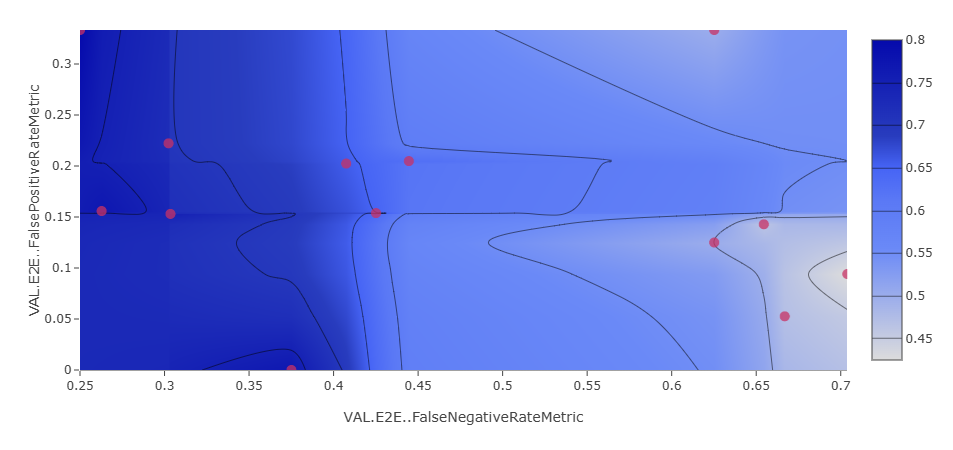
\includegraphics[width=\textwidth]{images/FNR-FPR-F1.png}
    \caption{Contour plot of FNR and FPR vs F1-Score. The darker the blue, the higher the F1-score.}
    \label{fig:fnrfpr}
\end{figure}

We assume that if LLMs do not have enough knowledge about particular configuration parameters, then they can not validate them. Therefore models that did not include these configurations in their training tend to invalidate configurations, because they are not aware of the existence of those parameters.

Next, we discuss the results of our RAG architectures. We had several configurations phases that included the following adaptations:
\begin{itemize}
    \item improving corpus data quality,
    \item changing retrieval types and their parameters,
    \item changing generation model,
    \item changing embedding model.
\end{itemize}

The bottleneck the pipeline appeared to be retrieval. In one of our later runs we were able to improve our results with dense retrieval by using an embedder that is especially good in coding and an advanced 4R architecture. However, this improvement was not sufficient to surpass the performance of newer standalone models (using the Ciri configuration). 

Resource preparation and data preprocessing are more valuable than blindly selecting a lot of models or system configurations. The results also showed that data cleanup for the corpus can lead to a decrease of retrieval quality in sparse and to an increase in retrieval quality for dense simultaneously. Improving retrieval quality is the most difficult part of enhancing configuration validation. Developing novel retrieval techniques or training a custom retrieval model are promising solutions to address the poor retrieval quality observed in configuration validation, but these approaches were outside the scope of our experiments. With sufficient monetary resources, one could test many different retrieval configurations with ease. However, our results suggest that small, specialized open-source embedding models (like \textit{infly/inf-retriever-v1-1.5b}) can be more suitable for this problem and also exhibit better performance regarding ingestion duration compared to the general-purpose proprietary embedding model tested (\textit{text-embedding-3-small}).

Even ignoring ingestion time, systems incorporating a retriever consistently required longer computation times and more RAM during runtime compared to the standalone baseline. Additionally, computation times were also model-dependent, as indicated by outliers for certain configurations in Figure \ref{fig:evaluation-time}.

\section{Threats to Validity} \label{sec:exp_threats}

This section discusses potential threats to the validity of the experimental findings presented in this chapter.

\paragraph{Internal Validity}
Internal validity refers to the extent to which the observed outcomes can be attributed to the experimental manipulations rather than extraneous factors.

\begin{itemize}
    \item \textbf{Baseline Reimplementation:} While efforts were made to faithfully replicate the Ciri system as a baseline, minor differences in our Haystack-based implementation compared to the original Ciri architecture could exist. These might subtly influence direct performance comparisons.
    \item \textbf{Documentation Corpus Integrity:} The web scraping process for documentation, while automated, might have encountered transient network issues or website structure changes leading to incomplete data or 404 errors for some pages. This could affect the completeness of the knowledge base for certain systems or versions.
    \item \textbf{API Reliability and Model Stability:} Reliance on external LLM APIs introduces a dependency on their uptime and consistent behavior. API errors or undocumented changes in underlying unversioned models (such as the most recent versions of \textit{gpt-4o-mini} or \textit{gemini-2.5-flash} used to test contemporary performance) could lead to failed queries or performance variations. While some of these failures might average out across many queries, they could also reflect issues with specific models or providers beyond our direct control.
    \item \textbf{System-Level Aggregation:} The decision to evaluate performance across all software systems in the CTest dataset, rather than per individual system (e.g., Django vs. Alluxio), was made for comparability and cost-efficiency. However, this aggregation might mask varying performance characteristics of the RAG configurations on specific systems.
    \item \textbf{LLM-as-a-Judge for Retrieval Metrics:} While we mitigated preference leakage by ensuring that the LLM judge (e.g., \textit{gpt-4o-mini}) was from a different family than the model generating the content being assessed for retrieval metrics where possible, the inherent subjectivity and potential biases of LLM judges remain an area of active research and could influence metrics like Context Relevance.
\end{itemize}

\paragraph{External Validity}
External validity concerns the generalizability of the experimental findings to other contexts.

\begin{itemize}
    \item \textbf{Corpus Specificity:} The document corpus was constructed specifically for the software systems and versions present in the CTest dataset. Therefore, the performance results, particularly for RAG configurations reliant on this corpus, may not directly generalize to newer software versions, different software systems, or entirely different documentation sets.
    \item \textbf{Task Scope:} This experiment focused on file-level configuration validation. The findings may not be directly applicable to parameter-level validation, inter-configuration dependency checking, or other types of software engineering tasks that might require different RAG strategies or knowledge representations.
    \item \textbf{Dataset Representativeness:} While CTest includes real-world and synthetic misconfigurations, the specific distribution and nature of these examples might not encompass all possible configuration errors or documentation complexities found in other operational environments.
\end{itemize}

\paragraph{Construct Validity}
Construct validity relates to how well the operationalizations (e.g., metrics, experimental setup) measure the intended theoretical constructs.
\begin{itemize}
   \item \textbf{Metrics for Validation Quality:} Standard classification metrics (F1-score, precision, recall) were used. While informative, they might not fully capture nuanced aspects of validation quality, such as the interpretability or actionability of the reasoning provided alongside a "valid" or "invalid" judgment. We used F1-Score for all conclusions for better comparability with the Ciri paper.
\end{itemize}

\section{Conclusion} \label{sec:exp_conclusion}
% Summarize the main findings and contributions of this specific experiment.
% Reiterate the performance of the best RAG system found.

We showed that configuration validation is still a difficult task for LLMs or RAGs. We did not exceed the results of the Ciri team with any RAG configuration. In our experiments, retrieval appeared to be the primary bottleneck. Retrieving up-to-date documentation pages for system configurations does not function effectively using standard BM25, a general-purpose embedding retriever, or even the specialized one we tested. Retrieval techniques and parameters such as hybrid retrieval did not have a large impact on retrieval quality. Future work could include metadata filtering, custom retrieval models, more advanced rewriting or adaptive RAG systems (also known as agentic), which were not in our scope.

We showed that more recent models are more capable of correctly validating configurations, but we also observed that their performance varies, and the results are not yet as reliable as needed for this task. We updated the Ciri experiment with more recent models; however, we could not establish a new state of the art result. Ciri's highest F1-score (0.790) was reported with Claude-3-Sonnet, a model not accessible during our experiments. Our application of DeepSeek's \textit{DeepSeek-chat-v3-0324} model using the Ciri configuration yielded a comparable F1-score of 0.776.